\chapter{Structure of our Agda files}
\par We have written 32 agda files with a total of 5785 lines of
code including comments and blank lines. These files can be divided into three categories:
1) definitions, 2) translation algorithms and 3) correctness
proofs. All the translation algorithms are inside the
\textbf{Translation} directory while the correctness proofs are inside
the \textbf{Correctness} directory. The other files belong to the
first category. Here is a simplified dependency graph of the files:

\begin{center} 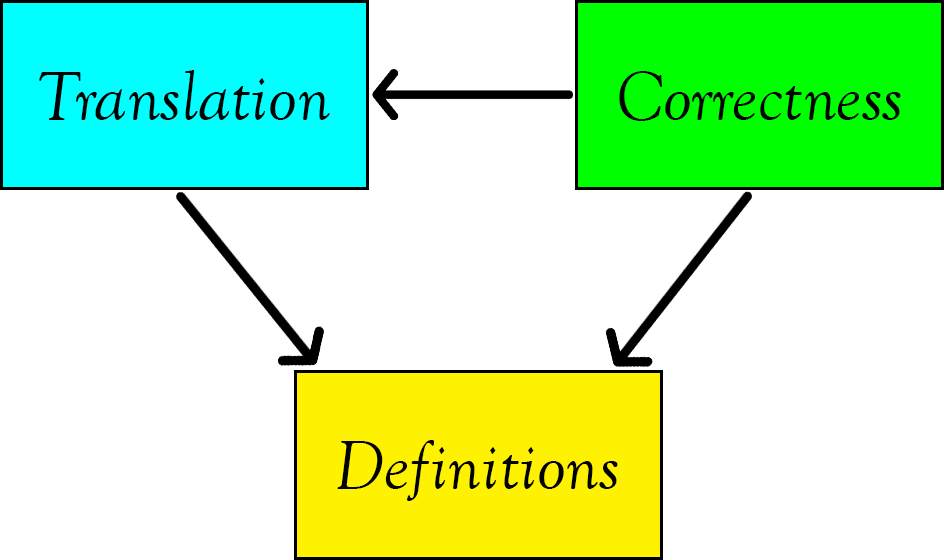
\includegraphics[width=.5\textwidth]{dependency} \end{center}

\par Readers are recommended to start with \textbf{Parsing-Regular-Expressions-in-Agda.agda}
,which is the index file of our formalisation. Now, let us look into each of the agda files. 

\begin{center}
\begin{longtable}{| p{5.2cm} | p{8.3cm} |}
\hline
\textbf{Parsing-Regular-Expressions-in-Agda.agda} & is the index
file of the Agda formalisation which imports all the other agda
files. Once this file has been compiled, all the other files will have been compiled as
well. \\ \hline 
\textbf{Subset.agda} & contains the definition and operations of subset. \\
  \hline
\textbf{../DecidableSubset.agda} & contains the definition and operations
                              of decidable subset. \\ \hline
\textbf{../VectorRep.agda} & contains the vector representation of sets. \\
  \hline
\textbf{Language.agda} & contains the definition and operations of language. \\
  \hline 
\textbf{RegularExpression.agda} & contains the definition of regular expression
                         and regular language. \\ \hline
\textbf{eNFA.agda} & contains the definition, operations and properties of
       \(\epsilon\)-NFA. \\ \hline
\textbf{NFA.agda} & contains the definition, operations and properties of
       NFA. \\ \hline
\textbf{DFA.agda} & contains the definition, operations and properties of
       DFA. \\ \hline
\textbf{MinimalDFA.agda} & contains the definition of minimal DFA. \\
  \hline 
\textbf{State.agda} & contains the state construction algorithm for
                      translating regular expressions to
                      \(\epsilon\)-NFA. \\ \hline
\textbf{Quotient.agda} & contains the quotient set construction
                         function for translating DFA to MDFA. \\
  \hline 
\textbf{RelationTable.agda} & contains the matrix representation of
                              a binary relation. This file is not
                              completed and thus it is not used in any
                              other files. \\ \hline
\textbf{Translation.agda} & is the index file of all the translation
                       algorithms. \\ \hline
\textbf{../RegExp-eNFA.agda} & contains the translation function
                                   \textbf{regexTo\(\epsilon\)-NFA} from regular
                                   expressions to \(\epsilon\)-NFA. \\
  \hline
\textbf{../eNFA-NFA.agda} & contains the translation function
                                   \textbf{remove-\(\epsilon\)-step}
                                from \(\epsilon\)-NFA to NFA. \\
                                \hline
\textbf{../NFA-DFA.agda} & contains the translation function
                                   \textbf{powerset-construction}
                                from NFA to DFA. \\
                                \hline
\textbf{../DFA-MDFA.agda} & contains the translation function
                                   \textbf{minimise}
                                from DFA to MDFA. \\
                                \hline
\textbf{../TableFillingAlgorithm.agda} & contains the algorithm
that computes the relation of distinguishable states. This file is not
completed and thus it is not used in any other files. \\
                                \hline
\textbf{Correctness.agda} & is the index file of all the correctness
                       proofs. \\ \hline
\textbf{../RegExp-eNFA.agda} & contains the proof that \(\forall
e\in RegExp.\ L(e) = L(regexTo\epsilon\)-NFA \(e)\). \\ \hline
\textbf{../../Epsilon-lemmas.agda} & contains the
\(\epsilon\) case of the above proof. \\ \hline
\textbf{../../Singleton-lemmas.agda} & contains the
\(\sigma\ a\) case of the above proof. \\ \hline
\textbf{../../Union-lemmas.agda} & contains the
union case of the above proof. \\ \hline
\textbf{../../Concatenation-lemmas.agda} & contains the
concatenation case of the above proof. \\ \hline
\textbf{../../KleenStar-lemmas.agda} & contains the
kleen star case of the above proof. \\ \hline
\textbf{../eNFA-NFA.agda} & contains the proof that \(\forall
enfa\in \epsilon\)-NFA\(.\ L(enfa) = L(remove\hyphen\epsilon\hyphen
step\ enfa)\). \\ \hline
\textbf{../NFA-DFA.agda} & contains the proof that \(\forall
nfa\in\)NFA\(.\ L(nfa) = L(powerset\hyphen construction\ nfa)\). \\ \hline
\textbf{../DFA-MDFA.agda} & contains the proof that \(\forall
dfa\in\)DFA\(.\ L(dfa) = L(minimise\ dfa)\). \\ \hline
\textbf{RegExp-Decidability.agda} & contains the proof of the
decidability of regular expressions. \\ \hline
\textbf{Example.agda} & contains an example on the recognition of a
string by a regular expression. \\ \hline
\textbf{Util.agda} & contains miscellaneous definitions and proofs
such as decidable equality. \\ \hline
\end{longtable}
\end{center}

\par We have also generated html files from the agda files. They are located in the \textbf{web} directory. Readers are
recommended to read the html files as it is much more
convenient. Similarly, readers can start with the
\textbf{Parsing-Regular-Expressions-in-Agda.html} which contains all
the links to other files. 